\documentclass[aspectratio=169]{beamer}
\usepackage[utf8]{luainputenc}
\usepackage{amssymb,amsmath}
\usepackage{graphicx}
\usepackage{tikz}
\usepackage{beamercolorthemetud}
\usepackage[backend=biber]{biblatex}
\usepackage{caption}
\captionsetup[figure]{font=scriptsize}
\usepackage{hyperref}

\usepackage{subcaption}
\usepackage[absolute,overlay]{textpos}
  \setlength{\TPHorizModule}{1mm}
  \setlength{\TPVertModule}{1mm}




\addbibresource{bibl.bib}
\setbeamertemplate{bibliography item}{\insertbiblabel}
\usepackage[english]{babel}
\usetheme[]{tud}
\setbeamercolor{background canvas}{bg=}
\setbeamerfont{frametitle}{size=\Large}
\input{macros}



\title{MeetForSport: Adaptation Concept}
\author{Mattis Lahr, Felix Fischer}
\date{10.12.2021}

\einrichtung{\hspace{-1pt}Institute of Systems Architecture}
\datecity{Dresden}




\AtBeginSection[]{\partpage{\usebeamertemplate***{part page}}}
\begin{document}
\maketitle



\begin{frame}
    \frametitle{Table of Contents}
    \tableofcontents
\end{frame}



\section{Hook}
\begin{frame}
\frametitle{App Idea}
This app will allow users to join group activities (i.e. football) or join ongoing events.
Targeting mostly active persons, this small social network will allow users  to find new friends/persons with the same interests and therefore allow these people to become more active.
\end{frame}

\section{Need}
	\begin{frame}
		\frametitle{Use Cases}
	\end{frame}

	\begin{frame}
		\frametitle{Challenges and need for Adaptation}
		\begin{columns}
		  \column{0.4\linewidth} 
			\begin{itemize}
				\item build/find an efficient way to find locations
				\item assign each sport a set of requirements (e.g. important features the location needs)
				\item build a database for users and events
			\end{itemize}
			 \column{0.6\linewidth}   
			 \begin{figure}
				 \centering
				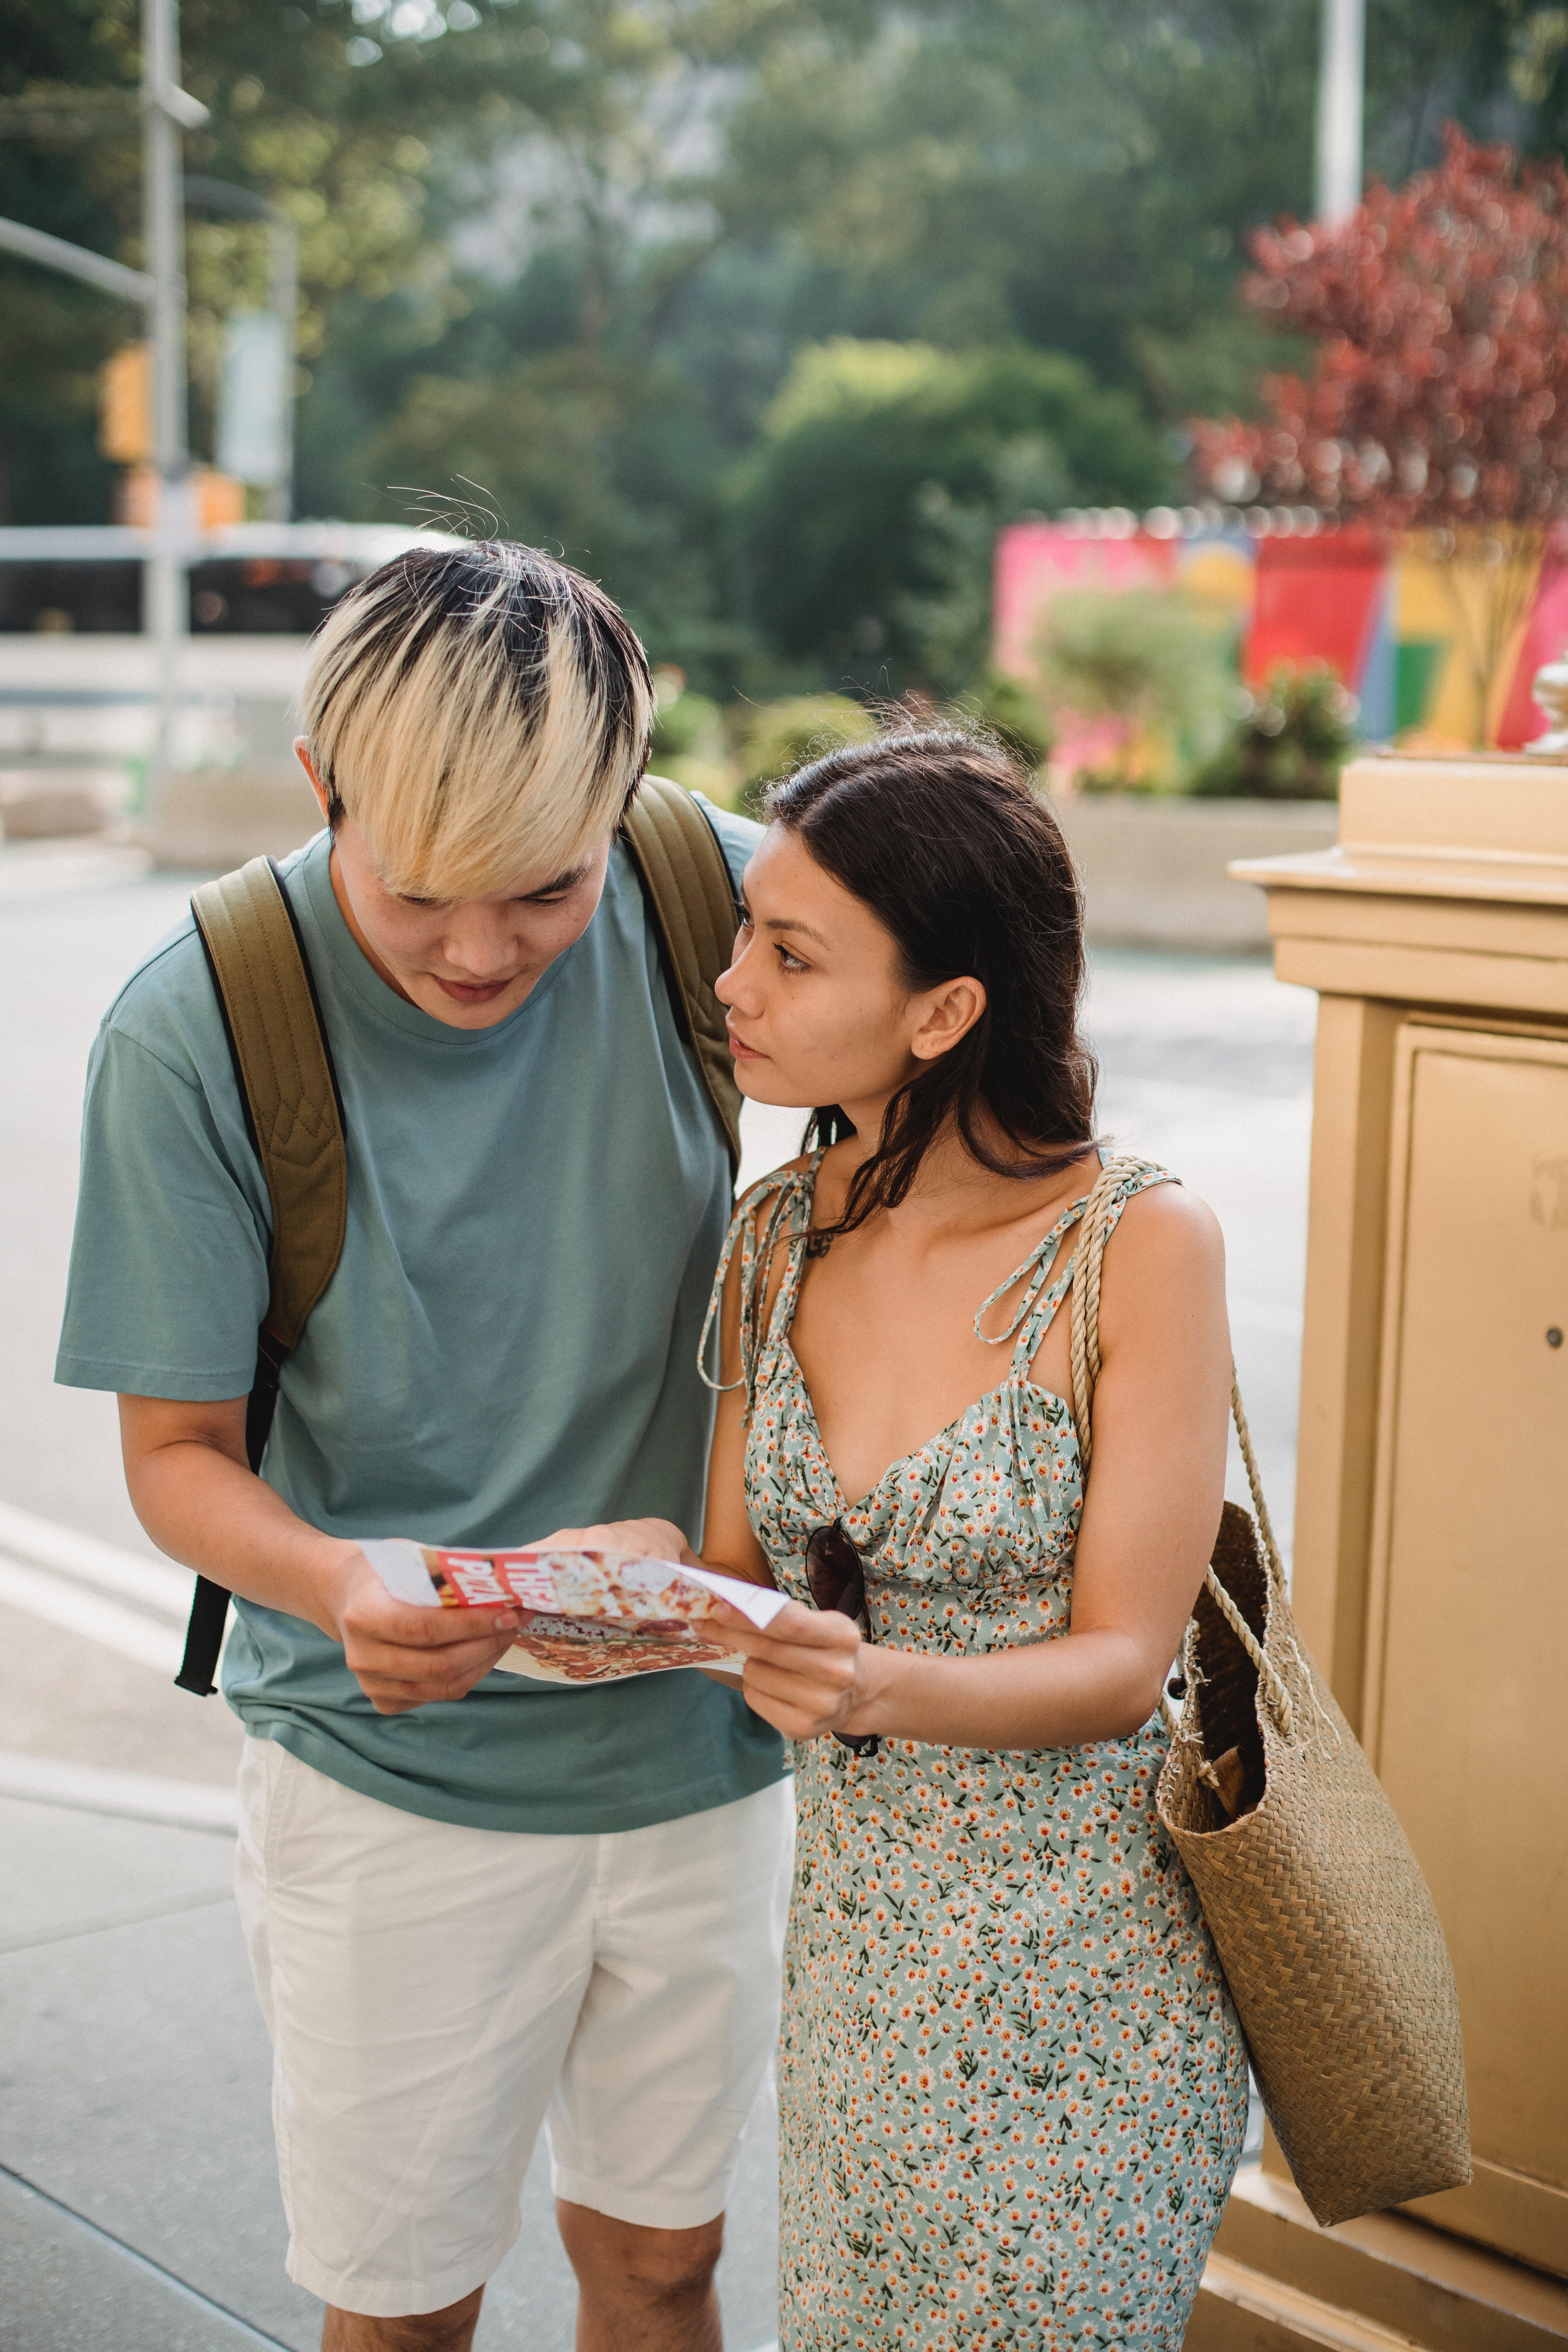
\includegraphics[width=0.5\textwidth]{media/no_gps.jpg}
			\end{figure}
		\end{columns}
	\end{frame}
	
	\begin{frame}
		\frametitle{Challenges and need for Adaptation}
		\begin{columns}
		  \column{0.4\linewidth} 
			\begin{itemize}
				\item build an organizer 
				\item implement interaction possibilities
				\item find a way to offer event information offline (connectivity challenge)
			\end{itemize}
		\column{0.6\linewidth}   
			 \begin{figure}
			 \centering
			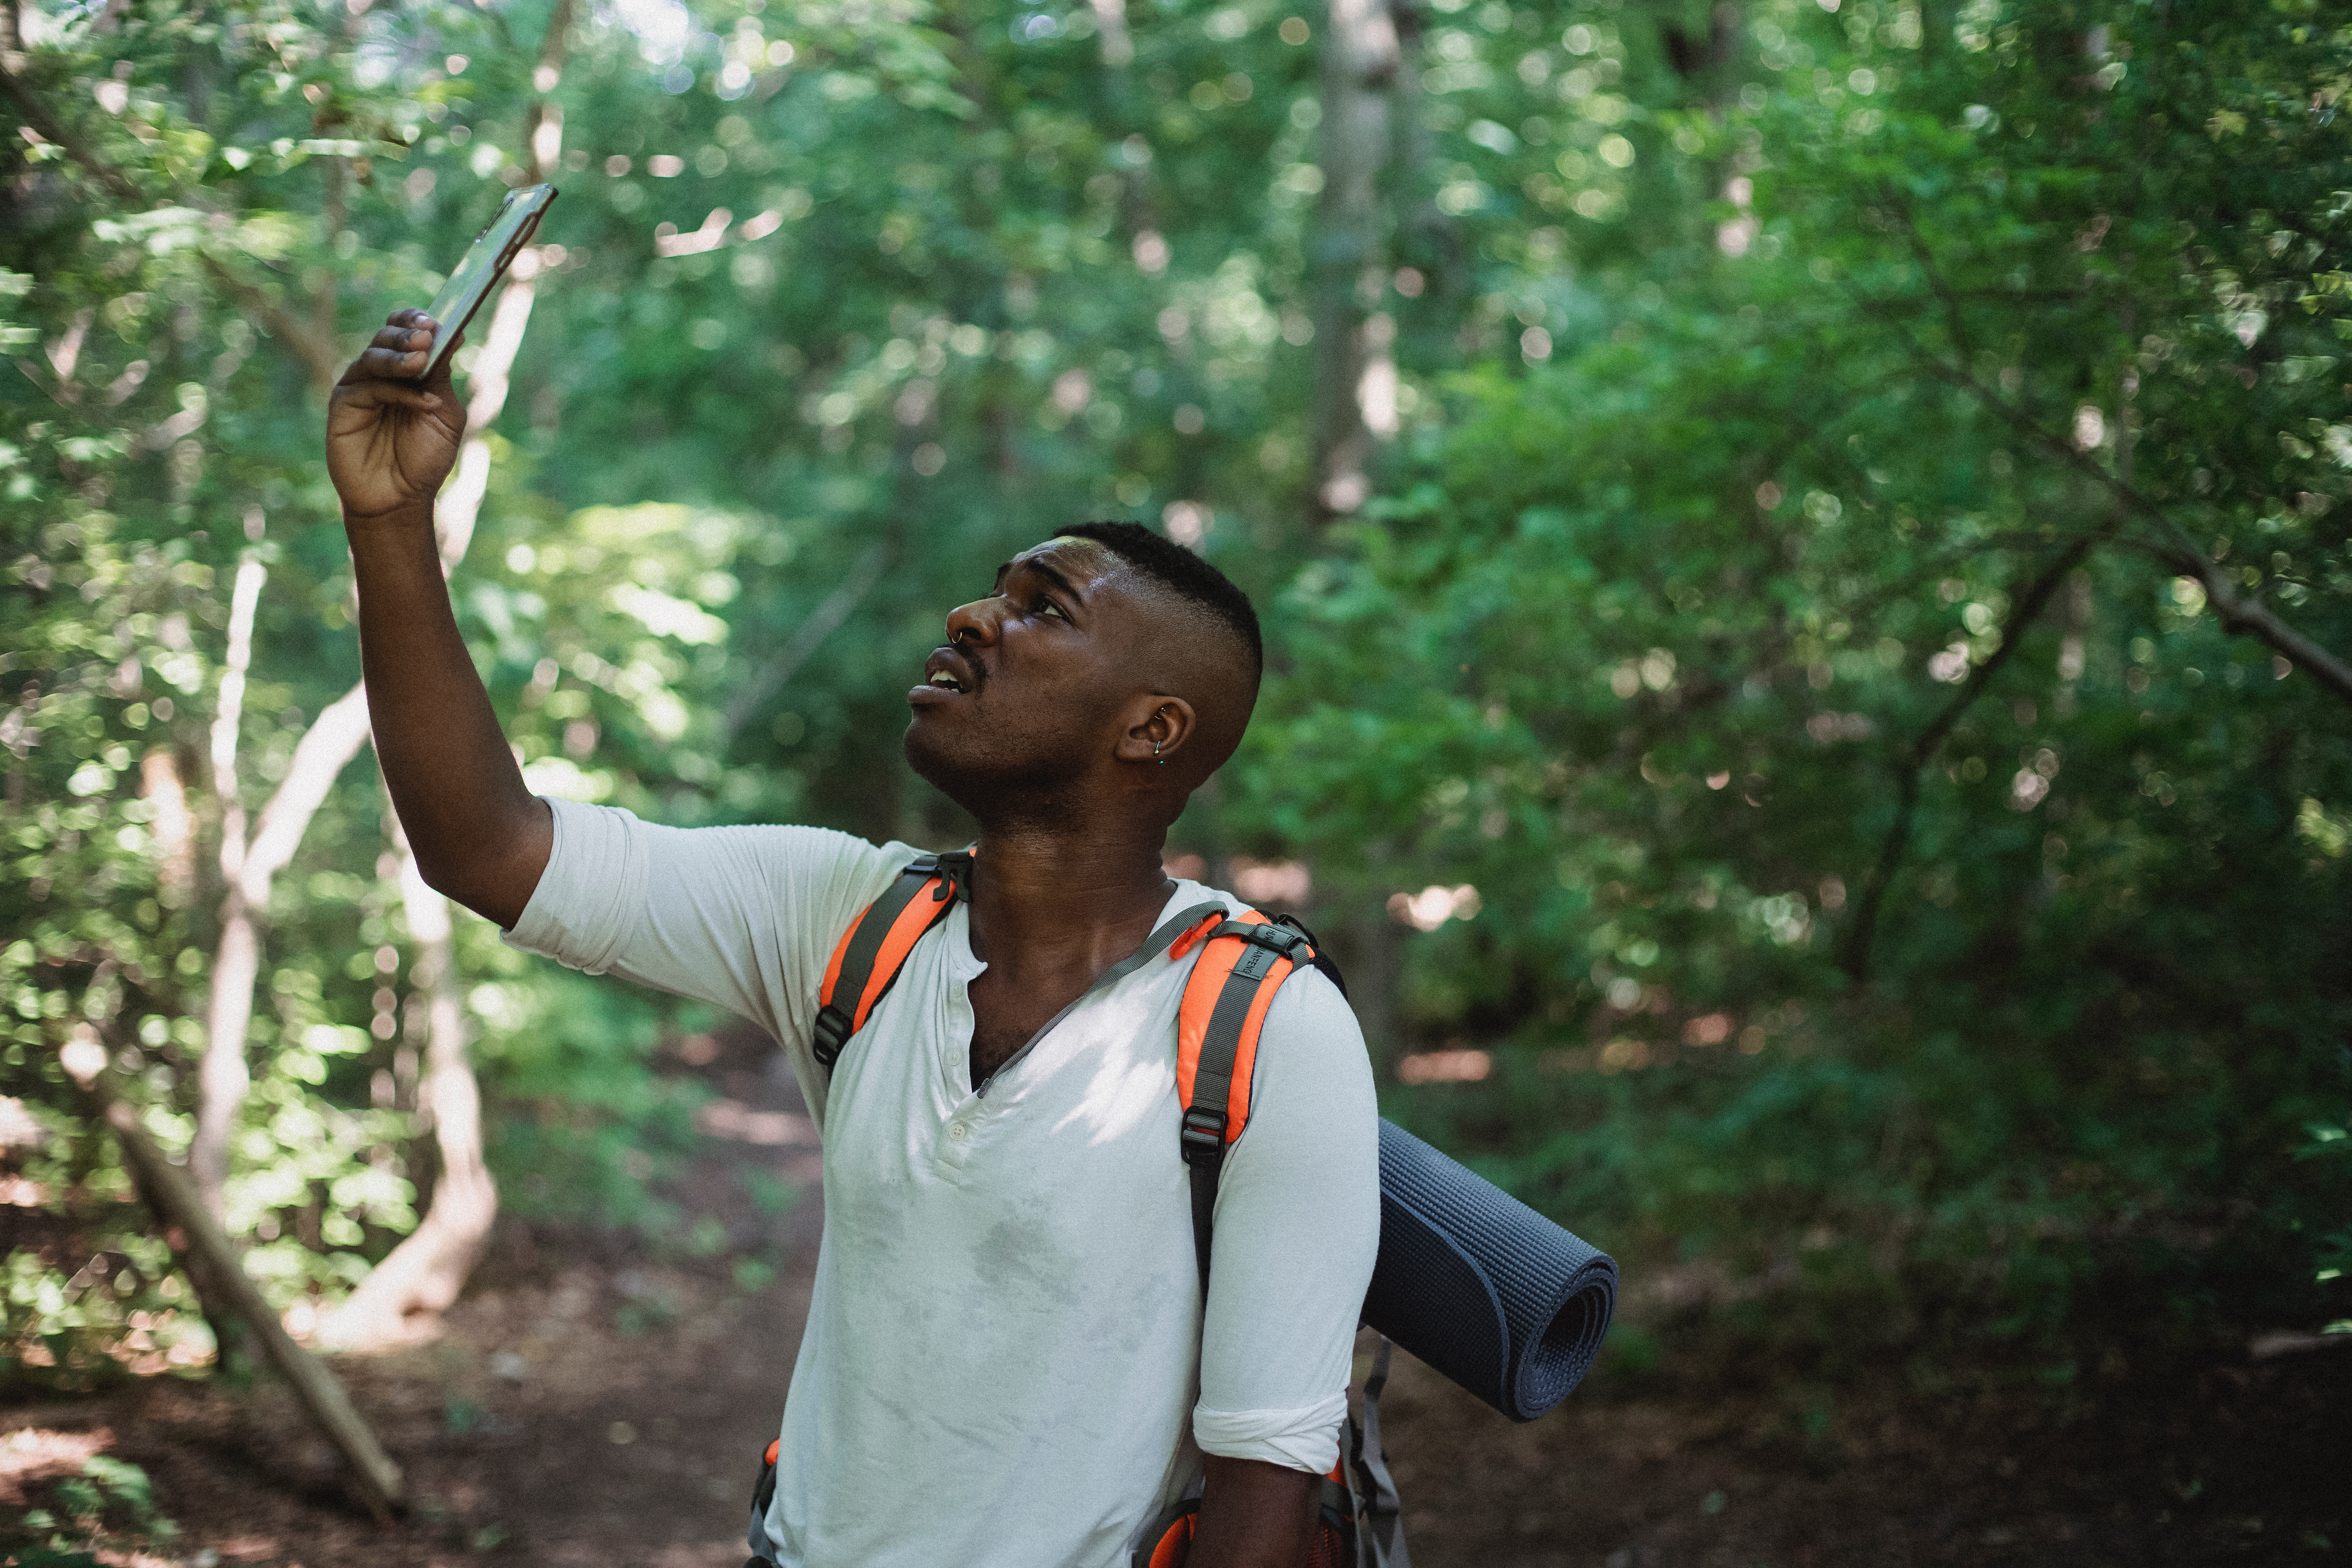
\includegraphics[width=1\textwidth]{media/no_internet.jpg}
		\end{figure}
		\end{columns}
	\end{frame}

\section{Approach}

	\begin{frame}
		\frametitle{Main Features}
		\begin{itemize}
			\item Creation of own events and joining into events of other users
			\item A filterable list of upcoming events
			\item An interactive map that displays event locations
		\end{itemize}
	\end{frame}

	\begin{frame}
		\frametitle{Adaptation Concepts}
		\begin{itemize}
			\item Detection and adaptation to bad or no internet
			\item Detection and adaptation to a low battery
		\end{itemize}
	\end{frame}

	\begin{frame}
		\frametitle{Architecture}
		 \begin{figure}
			\centering
			\includegraphics[width=0.8\textwidth]{media/architecture.jpg}
		\end{figure}
	\end{frame}

\section{Benefits}

	\begin{frame}
		\frametitle{Benefits}
		\begin{itemize}
			\item Easy social networking for a specific situation
		\end{itemize}
	\end{frame}

\section{Team}

	\begin{frame}
		\frametitle{Team}
		\begin{itemize}
			\item Felix Fischer - Backend 
			\item Mattis Lahr - Frontent
		\end{itemize}
	\end{frame}

\end{document}